\section{Actividad 14}

\subsection*{a) Iniciar GNU Radio, abrir y analizar el archivo \texttt{Modulador\_FM.grc}, ¿qué función implementa? Ejecutar y verificar visualmente el número de frecuencias laterales significativas para al menos 
5 valores distintos de $\beta$. Probar distintas configuraciones en cuanto a la señal de mensaje y la desviación máxima. Verificar los resultados observados en la simulación y contrastarlos con lo visto en las clases teóricas. Informar sobre lo observado.}

      \begin{figure}[H]
        \centering
        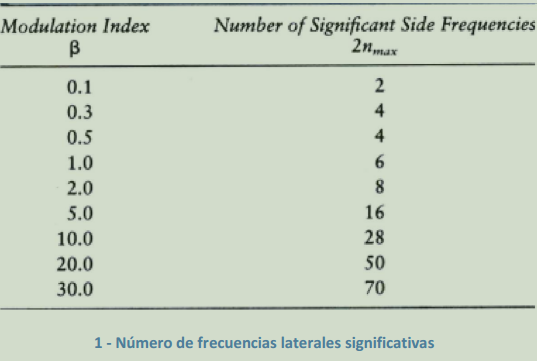
\includegraphics[width=0.6\textwidth]{imagenes/Parte_2/Actividad_14/fig6.png}
        \label{fig:6}
     \end{figure}

El \texttt{Modulador\_FM.grc} implementa la función de modulación en frecuencia donde:

    \[
        s(t) = A_c \cos \left( 2 \pi f_c t + \Delta f \int m(t) \, dt \right)
    \]

\begin{itemize}
    \item $m(t)$: señal modulante senoidal de 10 kHz.
    \item $f_c$: frecuencia portadora (100 kHz).
    \item $\Delta f$: desviación de frecuencia (controlada por el bloque \textit{Multiply Const} y el parámetro \texttt{deltaF}).
\end{itemize}

En el \textbf{QT Time Sink} se observó que la señal modulada (en rojo) presentaba una frecuencia instantánea variable en función de la amplitud de la señal modulante (en azul). Esto demuestra que la frecuencia de la portadora varía de manera proporcional al valor instantáneo del mensaje, lo que confirma el principio de la modulación en frecuencia.

En el \textbf{QT Frequency Sink} se visualizó el espectro de la señal modulada, donde fue posible identificar la portadora en $f_c$ y las componentes laterales ubicadas simétricamente a ambos lados de ella, separadas por múltiplos de la frecuencia de la señal modulante $f_m$.

Para el caso de $\beta = 0.3$, las principales componentes observadas fueron:

\[
f_c \pm f_m \quad \text{y} \quad f_c \pm 2f_m
\]

lo cual coincide con la \textbf{tabla teórica de número de frecuencias laterales significativas}, que establece que para un índice de modulación de 0.3 existen \textbf{cuatro frecuencias laterales significativas} (dos a cada lado de la portadora).

Por lo tanto, el espectro presenta \textbf{cinco líneas principales}: la portadora y dos pares de frecuencias laterales.

Se realizaron simulaciones adicionales variando los parámetros de \textbf{desviación de frecuencia} ($\Delta f$) y de \textbf{frecuencia del mensaje} ($f_m$) con el fin de generar distintos valores del índice de modulación $\beta$.

Los resultados mostraron los siguientes comportamientos característicos:

\begin{itemize}
    \item \textbf{Al aumentar $\Delta f$ (manteniendo $f_m$ constante)}, el índice $\beta$ aumenta, lo que provoca un mayor número de bandas laterales y un \textbf{ensanchamiento del espectro}. La portadora pierde potencia relativa y la energía se distribuye entre más componentes.

    \item \textbf{Al aumentar $f_m$ (manteniendo $\Delta f$ constante)}, el índice $\beta$ disminuye, reduciéndose la profundidad de modulación y, por tanto, el número de laterales y el ancho de banda total.
\end{itemize}

Estos resultados se corresponden con la teoría de la modulación en frecuencia, donde el número de frecuencias laterales significativas y el ancho de banda total dependen directamente del índice $\beta$.


%=======================================================================================
\subsection*{b) Abrir y ejecutar en GNU Radio el archivo FM\_Comercial.grc. Verificar e informa lo observado sobre el espectro de Radio FM comercial distribución de canales, ancho de banda de los mismos, ancho de banda de guarda, etc.).}

Al analizar el espectro de radio FM comercial mostrado en las Fig. \ref{fig:ejercicio_14b1} y \ref{fig:ejercicio_14b2}, se observan los siguientes puntos:

\begin{itemize}
    \item \textbf{Distribución de canales}: El espectro abarca un rango de frecuencias entre aproximadamente 94 MHz y 101 MHz. Los picos más prominentes, como los encontrados en 94.797 MHz (-5.43 dB) y 97.936 MHz (-20.48 dB), indican la presencia de canales de FM comerciales. Estos picos sugieren que las estaciones de radio están distribuidas a lo largo de este rango, con una separación típica entre canales.
    
    \item \textbf{Ancho de banda de los canales}: En FM comercial, el ancho de banda de cada canal suele ser de aproximadamente 200 kHz, según el estándar de radiodifusión. Esto incluye la señal modulada y los componentes laterales. En el espectro, los picos tienen una base ancha que apoya esta estimación, aunque la resolución exacta depende del ajuste del equipo.
    
    \item \textbf{Ancho de banda de guarda}: El espacio entre los picos de las señales sugiere un ancho de banda de guarda de alrededor de 200 kHz, que es típico para evitar interferencias entre canales adyacentes en la banda FM comercial (88-108 MHz).
    
    \item \textbf{Niveles de potencia}: Los niveles relativos (dB) varían significativamente, con algunos picos alcanzando valores cercanos a -20 dB y otros más débiles, lo que indica diferencias en la potencia de transmisión o distancia desde la fuente.
    
    \item \textbf{Ruido y señales débiles}: Se observa una actividad de ruido constante a lo largo del espectro, con fluctuaciones menores entre -80 dB y -100 dB, lo que es normal en un entorno de radiofrecuencia.
\end{itemize}

\begin{figure}[H]
    \centering
    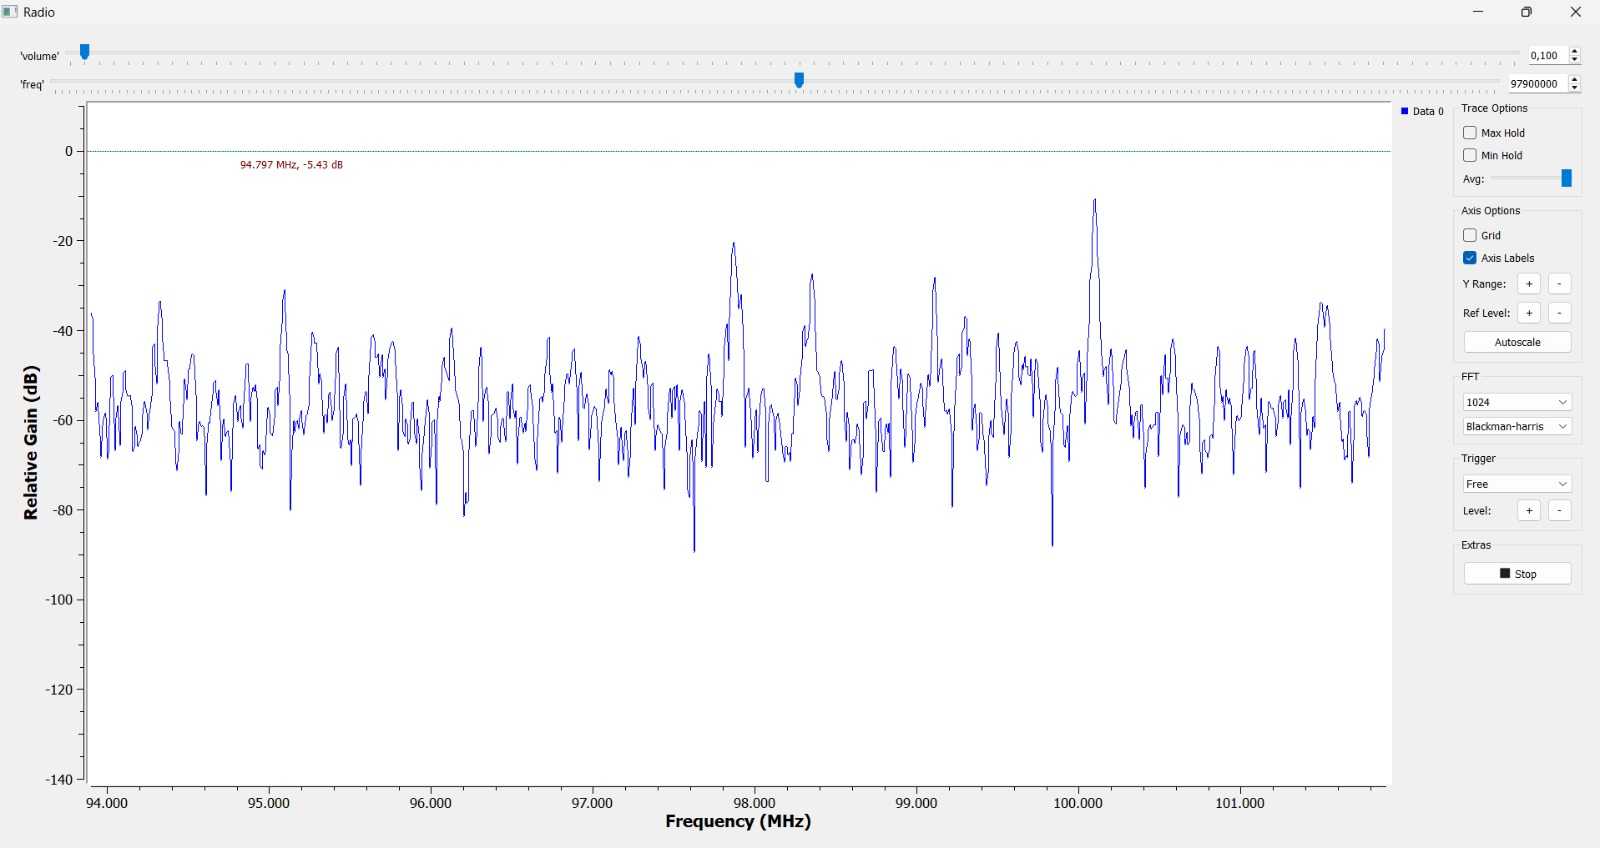
\includegraphics[width=0.9\linewidth]{imagenes/Parte_2/Actividad_14/14_b.jpg}
    \caption{Primera experimento.}
    \label{fig:ejercicio_14b1}
\end{figure}

\begin{figure}[H]
    \centering
    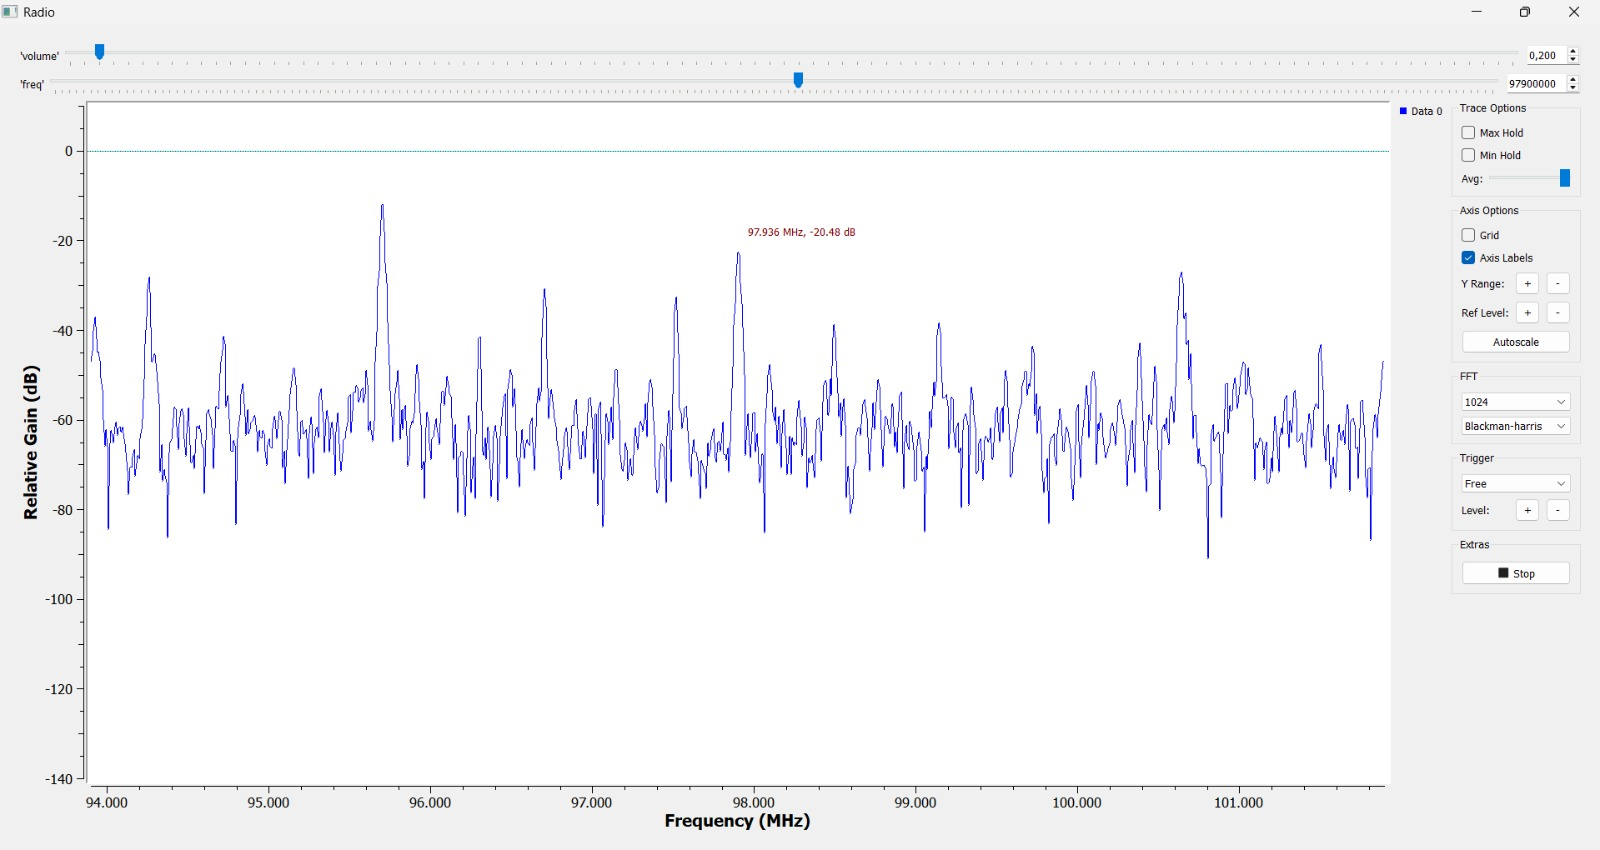
\includegraphics[width=0.9\linewidth]{imagenes/Parte_2/Actividad_14/14_c.jpg}
    \caption{Segundo experimento.}
    \label{fig:ejercicio_14b2}
\end{figure}

%=======================================================================================
\subsection*{d) Para desarrollar esta parte deberán trabajar entre dos grupos.}

\subsection*{1-  Abrir y ejecutar en una de las SDR el archivo FM\_Receptor.grc. Realizar lo mismo con el archivo FM\_Transmisor.grc en la otra SDR.}

\subsection*{2- Analizar y describir que realiza cada diagrama.}

El diagrama mostrado en el archivo \textbf{\texttt{FM\_Transmisor.grc}} representa un sistema transmisor de FM digital implementado en GNU Radio, donde la señal de audio modulante se convierte en una señal de radiofrecuencia modulada en frecuencia y transmitida mediante un dispositivo SDR (Osmocom Sink).

El bloque Signal Source (Audio) genera la señal modulante, una onda senoidal de baja frecuencia , que simula una señal de audio. Esta señal se combina con una portadora de RF generada por un bloque Signal Source (Coseno) y una frecuencia central ajustable (300 MHz) mediante el bloque Multiply Const. La modulación en frecuencia se logra aplicando la variación instantánea de la fase de la portadora en función de la amplitud de la señal del mensaje.

Los bloques Transcendental (cos y sin) generan las componentes en cuadratura (I y Q) necesarias para construir la señal compleja modulada en FM. Estas componentes son luego combinadas mediante los bloques Multiply y Subtract, y convertidas al formato complejo a través del bloque Float to Complex, produciendo así la señal modulada final.

Finalmente, la señal modulada es enviada al bloque Osmocom Sink, el cual transmite la señal de RF modulada en frecuencia a través del hardware SDR. Los bloques QT GUI Time Sink y QT GUI Frequency Sink permiten visualizar tanto el comportamiento temporal como espectral de la señal transmitida, verificando la correcta generación de la portadora y su desviación en frecuencia.

El diagrama mostrado en el archivo \textbf{\texttt{FM\_Receptor.grc}}  implementa un sistema básico de recepción de radio FM utilizando GNU Radio y un dispositivo SDR (Osmocom Source). El objetivo del esquema es capturar una señal de RF, realizar la conversión de frecuencia hacia una frecuencia intermedia o baseband mediante mezclado digital, filtrar la banda de interés y visualizar la señal resultante en el dominio del tiempo y la frecuencia.

La señal de RF es recibida por el bloque Osmocom Source, configurado con una frecuencia central de 300 MHz y una tasa de muestreo de 8 Msps. Esta salida se multiplica por una señal cosenoidal generada localmente (100 kHz) mediante el bloque Multiply, lo que produce una traslación espectral similar al proceso de heterodinación en un receptor superheterodino. Posteriormente, el filtro pasa bajos con una frecuencia de corte de 90 kHz elimina las componentes de alta frecuencia, dejando solo la banda útil correspondiente al canal FM seleccionado.

Los bloques QT GUI Time Sink y QT GUI Frequency Sink permiten visualizar la señal en los dominios temporal y frecuencial, verificando la correcta recepción y filtrado. Al variar los parámetros de frecuencia del SDR y del oscilador local, se puede sintonizar diferentes emisoras o desplazar la frecuencia intermedia.

\subsection*{3- Sintonizar en el receptor la misma frecuencia usada en el transmisor (verificar que la frecuencia utilizada se encuentre fuera del espectro comercial FM). Observar qué sucede con el espectro. Probar distintas distancias entre las SDR. Informar lo observado.}

Al sintonizar al receptor con la misma frecuencia usada en el transmisor se puede apreciar un pico en el espectro en dicha frecuencia, esto se logra apreciar en la Fig. \ref{fig:14_tonoDectectado}, a medida que la distancia entre el transmisor y receptor aumenta dicho pico en dicha frecuencia disminuye y esto se logra apreciar en la Fig. \ref{fig:14_tonoAleajndose}, mientras mas grande es la distancia entre ambos, el tono simple se va perdiendo.

    \begin{figure}[H]
        \centering
        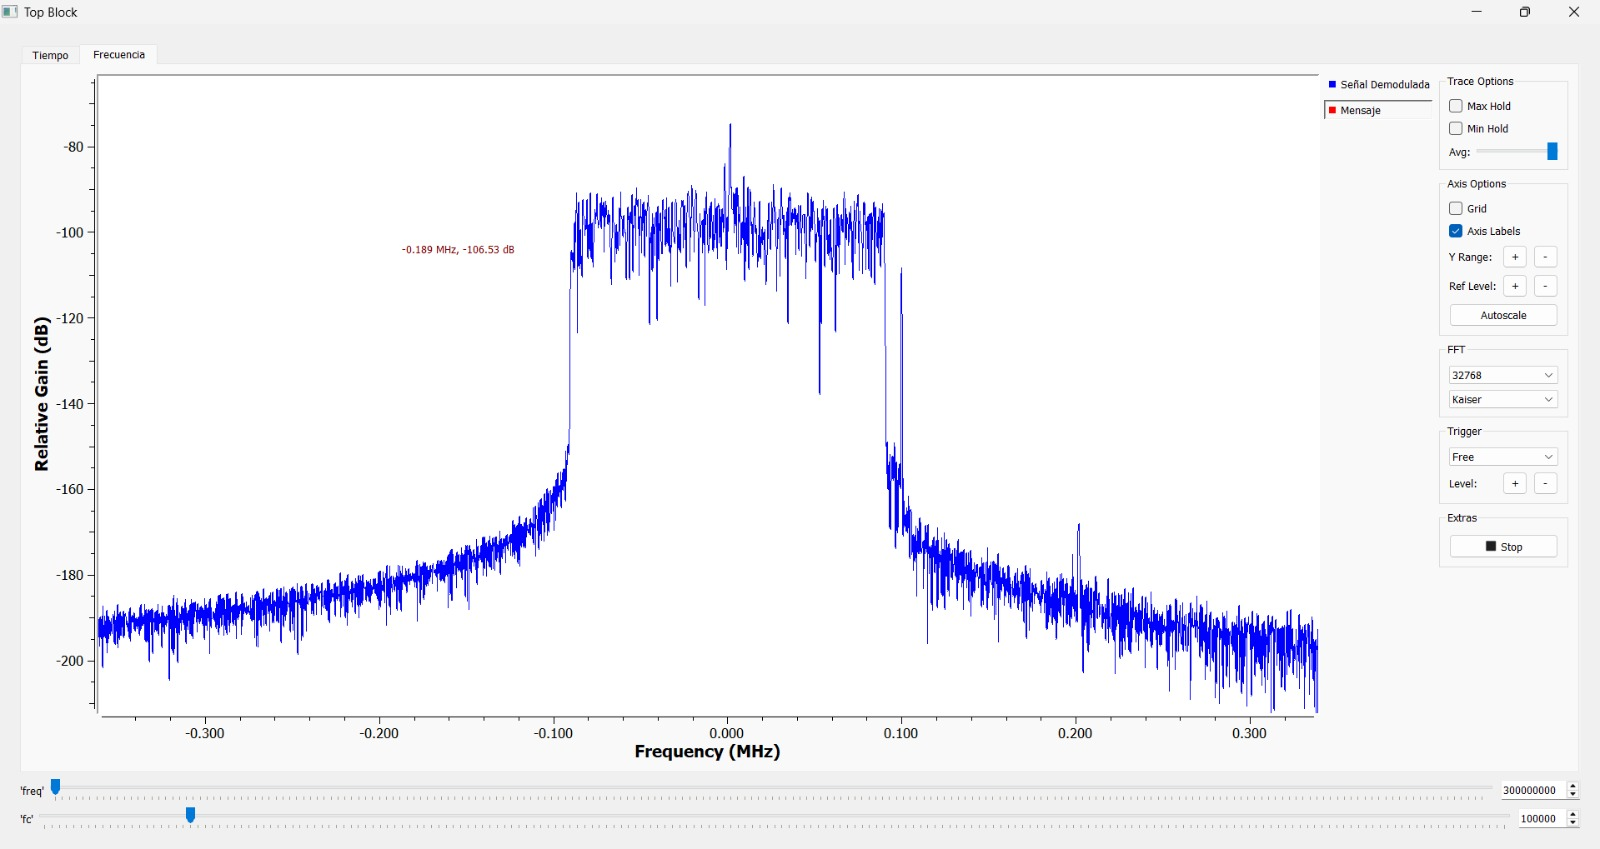
\includegraphics[width=0.9\linewidth]{imagenes/Parte_2/Actividad_14/14_tonoDetectado.jpg}
        \caption{Tono simple detectado.}
        \label{fig:14_tonoDectectado}
    \end{figure}

    \begin{figure}[H]
        \centering
        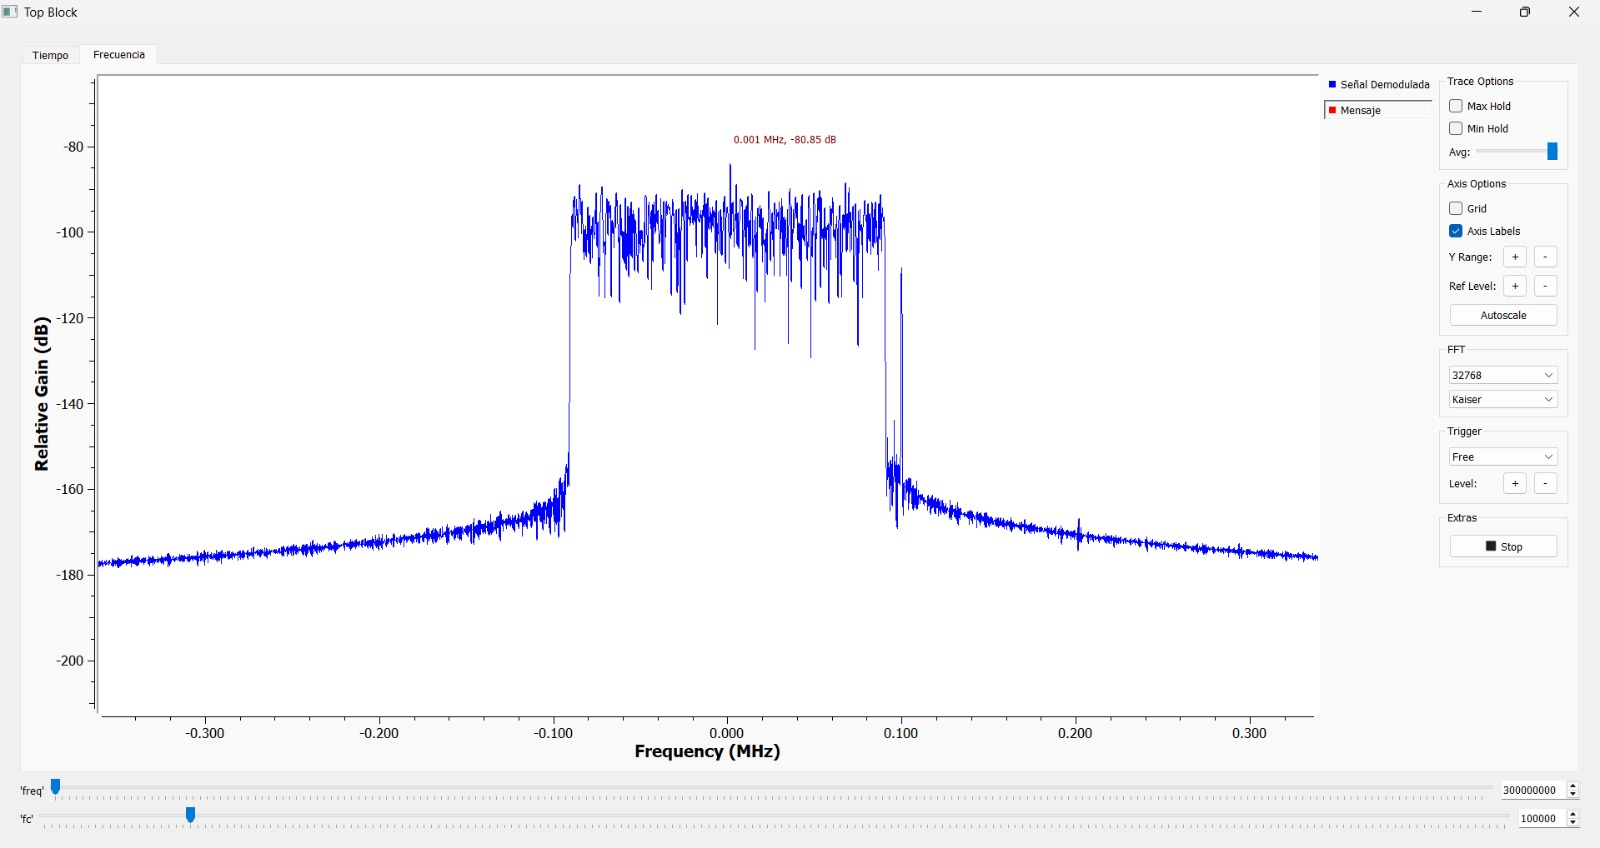
\includegraphics[width=0.9\linewidth]{imagenes/Parte_2/Actividad_14/14_tonoAlejandose.jpg}
        \caption{Aumenta distancia.}
        \label{fig:14_tonoAleajndose}
    \end{figure}